\documentclass[
  t,% place content on top of the page
]{_style/tudelft-beamerposter}

\usepackage[
  orientation=portrait,
  size=custom,
  width=76.2,
  height=101.6,
  scale=1.0,% was 1.4 in the template; 1.0 makes room for every section
]{beamerposter}

\usepackage{booktabs,tabularx,array}
\usepackage{qrcode}

% Dark "traditional poster" blue, used for the header bar, the section
% headings and the bullet markers. Change the hex code here to retune it.
\definecolor{posterblue}{HTML}{1F3A68}
\colorlet{primary}{posterblue}
% tag colour, the same blue as the figures: [D#] data, [M#] method, [R#] result
\definecolor{tagc}{HTML}{2A78D6}
\newcommand{\tg}[1]{\textcolor{tagc}{\textbf{[#1]}}}
% caption line under a figure or table
\newcommand{\capline}[2]{{\small\textbf{#1} #2}}

% used for the header bar, section headings, blocks etc.
\setbeamercolor{bars}{bg=posterblue, fg=white}
\setbeamercolor{structure}{fg=posterblue}

% ---------------- header contents ----------------
\newcommand{\courseline}{IE 643 Course Project}
\title[IE 643 poster]{Can a Language Model Draw a Network’s Graph from Code?}
\newcommand{\teamname}{Team Pensieve}
\author[Adarsh A Rao]{Adarsh A Rao}
\newcommand{\rollnumber}{24b2132}
\newcommand{\emailid}{adarsh.v0@iitb.ac.in}
\date{}

% Logo files (upload both to the Overleaf project, next to main.tex).
% logo.png is the IITB logo, IE643-Logo.pdf is the IE 643 course logo.
\newcommand{\leftlogo}{logo.png}
\newcommand{\rightlogo}{IE643-Logo.pdf}
% Height of both logos; the header grows or shrinks with it.
\newlength{\logoheight}
\setlength{\logoheight}{5cm}
% Each logo sits on a white rounded tile so it stays visible on the blue bar.
\newcommand{\logotile}[1]{%
  \tikz\node[fill=white, rounded corners=0.8cm, inner sep=0.6cm,
    minimum width=\logoheight+1.2cm, minimum height=\logoheight+1.2cm]
    {\includegraphics[height=\logoheight]{#1}};}
% ---------------------------------------------------

\institute[IIT Bombay]{}

\setlength{\columnsep}{0.1\linewidth}

\setlength{\TPHorizModule}{\paperwidth}
\setlength{\TPVertModule}{\paperheight}

\setbeamertemplate{footline}{}

% Header: blue bar with IITB logo | five centred white lines | IE 643 logo.
\renewcommand\maketitle{
  {\begin{beamercolorbox}[
    wd=\paperwidth,
  ]{bars}{%
    \vskip0.008\paperheight
    \hspace*{1cm}%
    % left: IITB logo
    \begin{minipage}[c]{0.15\paperwidth}\centering
      \logotile{\leftlogo}
    \end{minipage}\hfill
    % centre: the five lines of text, all in white
    \begin{minipage}[c]{0.62\paperwidth}\centering\robotoslab\color{white}
      {\Large\courseline}\\[0.006\paperheight]
      {\LARGE\inserttitle}\\[0.006\paperheight]
      {\large\teamname}\\[0.004\paperheight]
      {\normalsize\insertauthor\ (\rollnumber)}\\[0.002\paperheight]
      {\small\href{mailto:\emailid}{\textcolor{white}{\emailid}}}
    \end{minipage}\hfill
    % right: IE 643 course logo
    \begin{minipage}[c]{0.15\paperwidth}\centering
      \logotile{\rightlogo}
    \end{minipage}%
    \hspace*{1cm}
    \vskip0.008\paperheight
  }\end{beamercolorbox}}%
}

\begin{document}

\begin{frame}
  \maketitle

      \section*{Abstract}
  % Picture on the LEFT, text on the RIGHT. The layout is fitted automatically:
  % the picture is scaled to the exact height of the text (so it ends level
  % with the last line), and the text takes all the width the picture leaves,
  % minus \absgap. To change the look, only touch \absgap (space between
  % them) and \absstretch (how much wider than its true shape the picture may
  % be drawn: 1.00 = no stretching, 1.10 = 10% wider).
  \noindent\textbf{Task:} a large language model (LM) reads a network's class code and \texttt{forward()} method and writes the forward pass as a valid, drawable graph: layers, connections, nesting.

  % ------------------------------------------------------------------ Introduction
  % Table 1 on the LEFT, Figure 1 on the RIGHT, each with its caption.
  \section*{Introduction}
  \begin{minipage}[t]{0.52\linewidth}
    \vspace{0pt}\centering
    \capline{Table 1:}{Graphs right, \textbf{exact / lenient}, on real torchvision code. Lenient = the same
    computation written differently (layer settings left out, \texttt{F.relu} for \texttt{nn.ReLU},
    \texttt{a+b} for \texttt{b+a}).}\\[1ex]
    {\normalsize
    \begin{tabular}{@{}lcccc@{}}
      \toprule
      & \multicolumn{2}{c}{Flat format \tg{M1}--\tg{M7}} & \multicolumn{2}{c}{Hierarchical \tg{M8}--\tg{M9}}\\
      \cmidrule(lr){2-3}\cmidrule(l){4-5}
      & dev \tg{D3} & unseen \tg{D4} & dev blocks & dev nets \tg{D7}\\
      & 21 blocks & 17 blocks & 21 & 30\\
      \midrule
      1.5B, fine-tuned & 6 / 11 & 0 / 0 & 9 / 9 & 0 / 0\\
      14B, prompted & 1 / 4 & not run & 0 / 1 & 0 / 2\\
      1.5B + 14B, joined & 8 / 13 & not run & 9 / 10 & 0 / 2\\
      \bottomrule
    \end{tabular}}
  \end{minipage}\hfill
  \begin{minipage}[t]{0.48\linewidth}
    \vspace{0pt}\centering
    \includegraphics[width=0.9\linewidth]{figures/fig1_mc3.png}\\[1ex]
    \capline{Figure 1:}{Closest of the 17 unseen \tg{D4}, a video ResNet block (MC3): right but for one invented
    ReLU (orange). Blue: a 3D conv as one layer; \texttt{torch.fx} writes weight + \texttt{conv3d}, the same
    computation.}
  \end{minipage}

  % ------------------------------------------------------------------ Workflow (left) | Data table (right)
  % 0.42 + 0.54 is the split; keep them summing to about 0.96.
  \begin{minipage}[t]{0.35\linewidth}
  \vspace{0pt}
  \section*{Workflow}
  \centering
  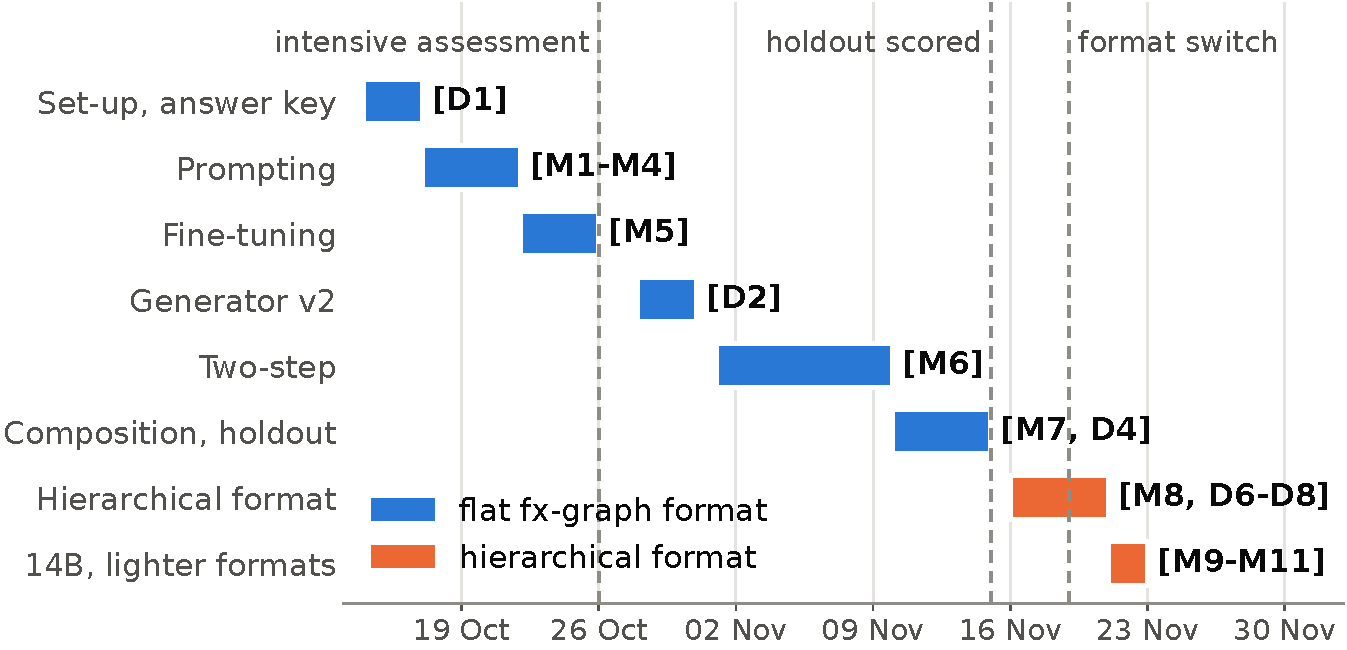
\includegraphics[width=\linewidth]{figures/gantt_poster.pdf}\\[0.5ex]
  \capline{Figure 2:}{Workflow, 14 Oct -- 22 Nov. Tags point to the data \tg{D} and methods \tg{M} below.}
  \end{minipage}\hfill
  \begin{minipage}[t]{0.65\linewidth}
  \vspace{0pt}
  \section*{Data}
  {\centering
  \capline{Table 2:}{Data sets. Graph size = nodes in the \texttt{torch.fx} graph, median (range).}\\[1ex]
  {\small\setlength{\tabcolsep}{4pt}
  \begin{tabularx}{\linewidth}{@{}l>{\raggedright\arraybackslash}Xlll@{}}
    \toprule
    Tag & What it is & Programs & Graph size & Role\\
    \midrule
    \tg{D1} & Generated, tiers 1--4 (generator v1) & 1{,}280 train, 40 test & 11 (7--25) & the basic skill\\
    \tg{D2} & Generated, tiers 5--6, library style (v1, then v2) & 640 train & 33 (8--119) & real-looking training code\\
    \tg{D3} & Real torchvision [5]: 18 blocks + 3 small networks & 21 & 14 (9--71) & development (``dev'')\\
    \tg{D4} & Real torchvision, 10 families never looked at (\emph{holdout}) & 17 & 16 (9--159) & locked, scored once\\
    \tg{D5} & Edits of D1 test programs: 69 change the graph, 124 do not & 193 & 12 (5--19) & does it follow the code?\\
    \tg{D6} & Hier.\ training: v3 (1{,}350) + tiers 1--4 (283) + \texttt{timm} (177) & 1{,}810 & nets 131 (22--2{,}684) & training\\
    \tg{D7} & Hierarchical dev: D3's 21 blocks + 30 whole torchvision networks & 51 & nets 177 (24--548) & development\\
    \tg{D8} & Hierarchical generated test (v3): 24 blocks + 51 networks & 75 & nets 109 (29--352) & generated test\\
    \tg{D9} & Hierarchical locked sets: unseen torchvision families + \texttt{timm} & 15 + 6 & up to 1{,}902 & not yet scored\\
    \bottomrule
  \end{tabularx}}\par}
  \end{minipage}

  \vspace{1ex}
 \noindent
\begin{minipage}[c]{0.68\linewidth}
  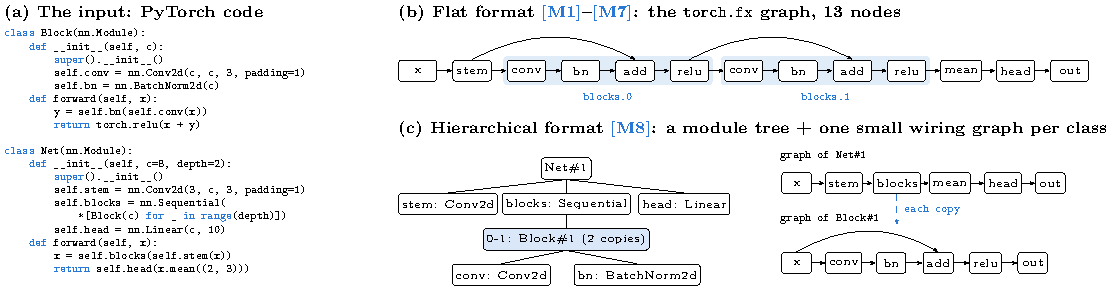
\includegraphics[width=\linewidth]{figures/fig3_demo.pdf}
\end{minipage}%
\hfill
\begin{minipage}[c]{0.29\linewidth}
  \capline{Figure 3:}{Demo: one program, both formats (real answer-key output). (b) repeats every block, so it
  grows with depth. (c) The tree says what is inside what and how many copies (\texttt{0-1: Block\#1}); each
  class is wired once.}\\[3ex]
  % Code QR sits here, in the space beside Figure 3, so it adds no height
  {\centering
  \textbf{Code}\\[1ex]
  \qrcode[height=5cm]{https://github.com/Rao-Adarsh/graphArt_LM}\\[1ex]
  {\footnotesize\url{https://github.com/Rao-Adarsh/graphArt_LM}}\par}
\end{minipage}

  % ------------------------------------------------------------------ Methods
  \section*{Methods}
  Models: Qwen2.5-Coder [3] 1.5B--14B, Gemma 31B; LoRA [2] (small add-on weights) on free Kaggle T4s.
  \textbf{Exact} = same operations wired the same way as \texttt{torch.fx} (labelled graph isomorphism);
  \textbf{lenient} also forgives notation (Table 1).\\[1ex]
  % three columns: flat methods | hierarchical methods | why the second format
  \begin{minipage}[t]{0.31\linewidth}
    \vspace{0pt}
    \textbf{Flat format -- the whole graph (Fig.~3b)}
    \begin{itemize}
      \item[\tg{M1}] \textbf{Zero-shot}: the code and the format rules only.
      \item[\tg{M2}] \textbf{Few-shot}: + worked examples from the training split.
      \item[\tg{M3}] \textbf{Chain of thought}: ``think step by step'' first [4].
      \item[\tg{M4}] \textbf{Chain of simulation}: track each variable's node [7].
      \item[\tg{M5}] \textbf{LoRA fine-tuning} (1.5B): whole graph in one go.
      \item[\tg{M6}] \textbf{Two-step}: nodes first, then edges naming variables.
      \item[\tg{M7}] \textbf{Composition}: one model lists, another wires.
    \end{itemize}
  \end{minipage}\hfill
  \begin{minipage}[t]{0.29\linewidth}
    \vspace{0pt}
    \textbf{Hierarchical format (from 19 Nov, Fig.~3c)}
    \begin{itemize}
      \item[\tg{M8}] \textbf{Tree + class graphs}: tree, then wiring; tuned 1.5B.
      \item[\tg{M9}] \textbf{Prompted 14B} on M8, with 2 worked examples.
      \item[\tg{M10}] \textbf{Per-instance trees}: one call per module, joined by code.
      \item[\tg{M11}] \textbf{Lighter formats}: same replies, scored for less.
    \end{itemize}
  \end{minipage}\hfill
  \begin{minipage}[t]{0.36\linewidth}
    \vspace{0pt}
    \textbf{The second format, and why (19 Nov)}
    \begin{itemize}
      \item Whole real networks are long in the flat format (median 177 nodes, up to 548; \texttt{timm} up to
      2{,}684), every repeated block written out again: too long for a 1.5B to write, or to train on with a T4.
      \item So we split the answer (Fig.~3c): a \textbf{tree} of modules (what is inside what, how many copies)
      and a small \textbf{wiring graph per class} ($\le$27 nodes), each written once. Repeats become a count;
      wiring stays local. Right only if the tree and every class graph are. New cost: the tree needs what the constructor
      builds.
    \end{itemize}
  \end{minipage}

  % ------------------------------------------------------------------ Results
  \section*{Results}
  % To be filled once the space left is known (candidates: report/novelty/figures/fig4_hier.pdf,
  \textbf{\tg{R1} Prompting \tg{M1}--\tg{M4} on \tg{D1}: size decides it.} Right topology:
  1.5B (5\%) $<$ 7B (25\%) $<$ 14B (60\%) $<$ 31B (93\%).\\[1ex]
  % R2 (figure) | R3 | R4
  \begin{minipage}[t]{0.33\linewidth}
    \vspace{0pt}
    \textbf{\tg{R2} Fine-tuning \tg{M5}: perfect at home, lost on real code}\\[0.5ex]
    \centering
    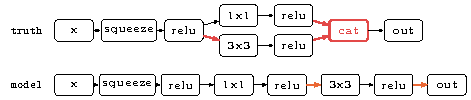
\includegraphics[width=\linewidth]{figures/fig4_fire.pdf}\\[0.5ex]
    \raggedright
    \capline{Figure 4:}{The 1.5B after LoRA: 40/40 on generated test code \tg{D1}, but \textbf{0/21} on real
    torchvision \tg{D3}. In figure: SqueezeNet's Fire block}
  \end{minipage}\hfill
  \begin{minipage}[t]{0.31\linewidth}
    \vspace{0pt}
    \textbf{\tg{R3} Real-looking data, then split the task \tg{D2}\tg{M6}\tg{M7}}
    \begin{itemize}
      \item The largest gain: training also on library-style code \tg{D2} took real blocks \tg{D3} from
      \textbf{0 to 7/21}.
      \item The task splits in two. The best lister names the right nodes on 15/21; given the true nodes, a
      tuned 1.5B wirer is right on 16/21. Joined \tg{M7}: \textbf{11/21}; 13/21 with the 14B as wirer.
    \end{itemize}
  \end{minipage}\hfill
  \begin{minipage}[t]{0.31\linewidth}
    \vspace{0pt}
    \textbf{\tg{R4} The locked test dataset \tg{D4}: 0/17 for every system}
    \begin{itemize}
      \item Even lenient, not one unseen block right; the closest is Fig.~1.
      \item The models fill gaps with guesses: library layers whose code is not in the prompt become one box
      (\texttt{Conv2dNormActivation} instead of conv $\rightarrow$ norm $\rightarrow$ activation)
    \end{itemize}
  \end{minipage}

  \vspace{1.5ex}
  % R5 text | Fig 5(a) | R6 text | Fig 5(b)
  \begin{minipage}[t]{0.21\linewidth}
    \vspace{0pt}
    \textbf{\tg{R5} Hierarchical \tg{M8}\tg{D6}--\tg{D8}: the tree is the bottleneck}\\[0.3ex]
    Real networks: 0/30; with the true tree given, 10/30. To write the tree the model must run the
    constructor in its head (loop counts, computed widths).
  \end{minipage}\hfill
  \begin{minipage}[t]{0.26\linewidth}
    \vspace{0pt}\centering
    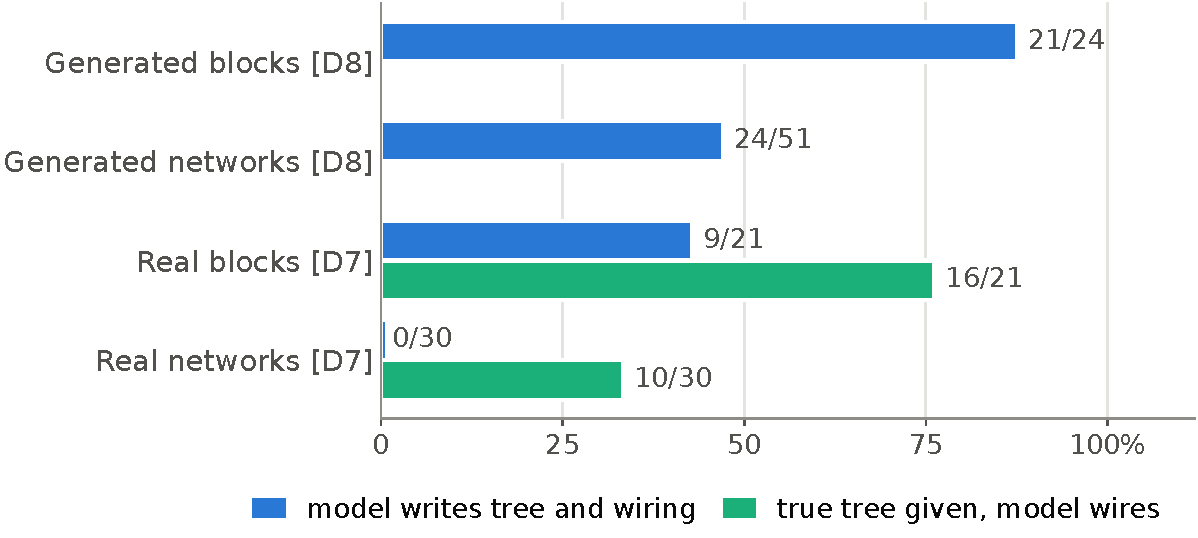
\includegraphics[width=0.9\linewidth]{figures/fig5a_hier.pdf}\\[0.3ex]
    \capline{Figure 5(a):}{Hierarchical drawings right; aqua: true tree given.}
  \end{minipage}\hfill
  \begin{minipage}[t]{0.21\linewidth}
    \vspace{0pt}
    \textbf{\tg{R6} Bigger model, less output \tg{M9}\tg{M11}}\\[0.3ex]
    Prompted 14B: trees no better (2/30 lenient). Asking for less: class graphs only (S0) gets
    \textbf{9/30} real networks, with 8$\times$ shorter output (found after the fact; to be scored on \tg{D9}).
  \end{minipage}\hfill
  \begin{minipage}[t]{0.26\linewidth}
    \vspace{0pt}\centering
    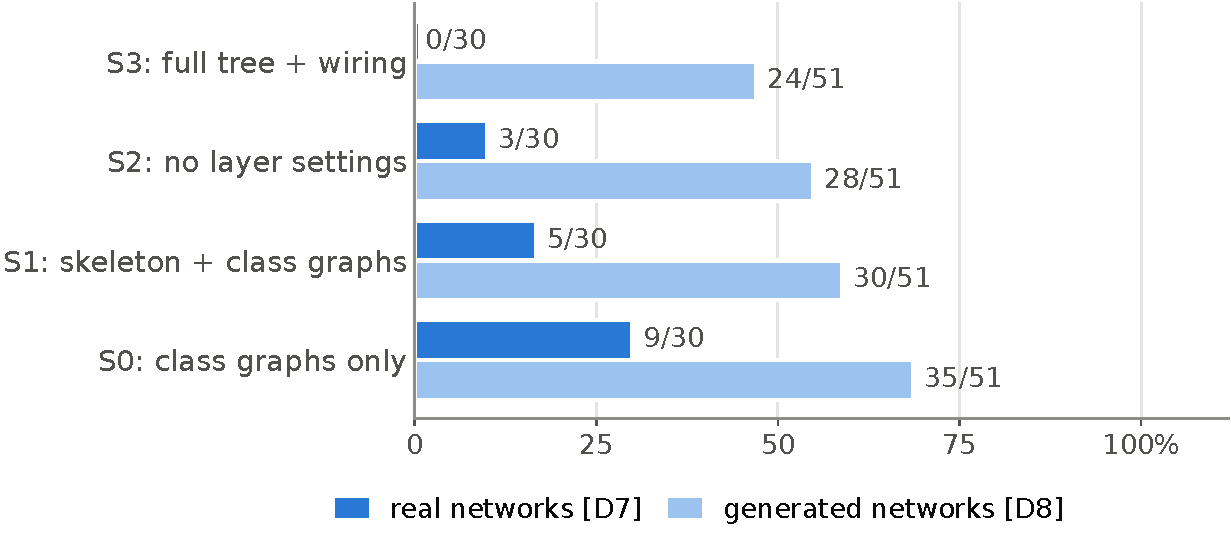
\includegraphics[width=0.9\linewidth]{figures/fig5b_lighter.pdf}\\[0.3ex]
    \capline{Figure 5(b):}{Same replies, lighter formats: S3 (all) to S0 (class graphs only).}
  \end{minipage}
  % the SqueezeNet Fire drawing, R1-R6 from the report).

  \end{frame}
\end{document}